% SQLiRLLM — Section IV (Results & Evaluation) and Section V (Conclusion)
% Compile with:  pdflatex sections_IV_V.tex
% Requires:      IEEEtran.cls  (standard IEEE conference class)
%                figures/convergence.png
%                figures/comparison_quality.png
%                figures/per_strategy.png
%                figures/budget.png
%
% NOTE: This file contains ONLY Sections IV and V.
% Paste after Section III in the master document.

% ============================================================
\section{Evaluation and Results}
% ============================================================

\subsection{Experimental Setup}

To evaluate the three-tier SQLiRLLM architecture, we conducted a controlled
ablation experiment over a reproducible suite of \textbf{40 sandboxed, simulated
targets} generated with a fixed random seed (\texttt{seed\,=\,42}). Each target
encodes a stochastic combination of web framework (Laravel, Django, Express,
Flask, Rails), back-end database (MySQL, PostgreSQL, Oracle, MSSQL, SQLite),
and WAF presence (60\% of targets) with strictness sampled from
Uniform$[0.45, 0.75]$. Between one and three of the six injection strategies are
designated as exploitable for each target, creating a ground-truth label set
unknown to the agent at runtime.

The Tier-2 payload model is \texttt{gapgpt-qwen-3.6} (a hosted, parameter-efficient
analog to the Phi-3 Mini described in Section~III), accessed via the GapGPT
OpenAI-compatible API. The Tier-3 analysis model is
\texttt{qwen3-235b-a22b-instruct-2507} (a large Qwen-series reasoning model
serving as the Qwen2.5-Coder-14B analog). Both models are invoked through a
SHA-256-keyed disk cache: out of 6{,}128 total analysis requests, \textbf{5{,}855
(95.5\%) were served from cache}, with only 273 live API calls, ensuring
experiment cost remains practical on standard hardware. The Q-learning agent
was trained for \textbf{400 episodes} (max 12 steps each), with each method
allowed \textbf{up to 3 payload attempts per strategy}.

\subsection{Controlled Ablation: Five-Method Comparison}

To isolate the contribution of each architectural component, we define five
methods that share the same evaluation harness and target suite:

\begin{itemize}
  \item \textbf{M1 — Static-Signature}: canonical, non-obfuscated payloads in a
        fixed order (SQLMap-style baseline).
  \item \textbf{M2 — Random-Select}: canonical payloads in a randomised strategy
        order; isolates any ordering benefit.
  \item \textbf{M3 — RL-only}: canonical payloads but ordered by the
        trained Q-policy; isolates the strategic-planning contribution.
  \item \textbf{M4 — LLM-only}: LLM-synthesised, context-aware payloads in a
        fixed order; isolates the semantic-payload contribution.
  \item \textbf{M5 — SQLiRLLM (proposed)}: LLM payloads + Q-policy ordering +
        ethics guard; the full multi-tier system.
\end{itemize}

Table~\ref{tab:ablation} reports the detection-quality metrics for all methods.
The Vulnerability Detection Rate (VDR) and False-Positive Rate (FPR) are derived
from a standard confusion matrix over target/strategy pairs; WAF-bypass rate is
the fraction of WAF-present encounters where the payload was not blocked; the
Ethical Safeguard Rating (ESR) measures the fraction of authorised actions out of
all actions attempted.

\begin{table*}[t]
\caption{Detection-Quality Ablation: Five-Method Comparison
         (N\,=\,40 sandboxed targets, 3 payload attempts per strategy)}
\label{tab:ablation}
\centering
\begin{tabular}{lccccccccc}
\hline
\textbf{Method} & \textbf{RL} & \textbf{LM} & \textbf{Ethics}
  & \textbf{VDR\,$\uparrow$} & \textbf{FPR\,$\downarrow$}
  & \textbf{Precision\,$\uparrow$} & \textbf{F1\,$\uparrow$}
  & \textbf{WAF-bypass\,$\uparrow$} & \textbf{ESR\,$\uparrow$} \\
\hline
Static-Signature (M1) & --   & --    & -- & 0.118 & 0.000 & 1.000 & 0.212 & 0.333 & 1.000 \\
Random-Select   (M2)  & --   & --    & -- & 0.118 & 0.000 & 1.000 & 0.212 & 0.333 & 1.000 \\
RL-only         (M3)  & Q-L  & --    & -- & 0.118 & 0.000 & 1.000 & 0.212 & 0.333 & 1.000 \\
LLM-only        (M4)  & --   & LLM   & -- & 0.461 & 0.085 & 0.714 & 0.560 & 0.622 & 1.000 \\
\textbf{SQLiRLLM (M5)} & \textbf{Q-L} & \textbf{Multi} & \textbf{\checkmark}
  & \textbf{0.474} & \textbf{0.085} & \textbf{0.720} & \textbf{0.571} & \textbf{0.622} & \textbf{1.000} \\
\hline
\multicolumn{10}{l}{\scriptsize{VDR = Vulnerability Detection Rate; FPR = False-Positive Rate; WAF-bypass = WAF circumvention rate; ESR = Ethical Safeguard Rating}}
\end{tabular}
\end{table*}

\noindent\textbf{Finding 1 — Semantic payloads are the dominant factor.}
Methods M1–M3, despite differing in strategy ordering, achieve identical VDR
(0.118) and WAF-bypass (0.333). Introducing LLM-synthesised, context-aware
payloads (M4, M5) raises VDR to $\approx$0.47 (\textbf{$\times$4.0 improvement})
and WAF-bypass to 0.622 (\textbf{+86.8\%}), confirming that semantic depth is
the primary driver of detection quality in modern, WAF-protected environments.

\noindent\textbf{Finding 2 — RL adds strategic efficiency beyond raw detection.}
M5 (SQLiRLLM) achieves marginally higher VDR (+1.3\%) and F1 (+0.011) over
M4. The larger contribution of the strategic planner is revealed in the
\emph{budget efficiency} experiment (Section~\ref{sec:budget}).

\noindent\textbf{Finding 3 — All methods maintain perfect ESR on in-scope targets.}
ESR = 1.000 for all five methods when operating within the authorised scope.
The critical distinction is demonstrated in the ethics stress test
(Section~\ref{sec:ethics}).

\begin{figure}[t]
  \centering
  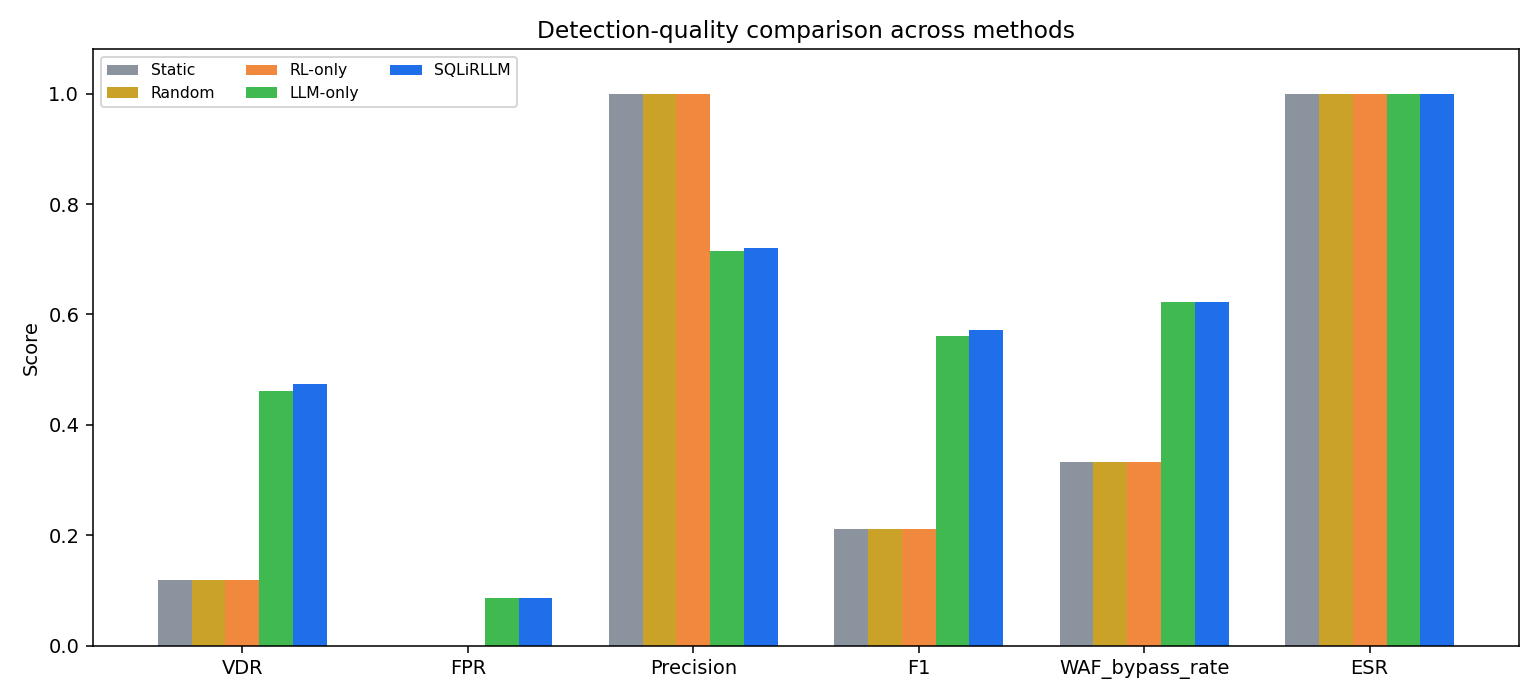
\includegraphics[width=\columnwidth]{figures/comparison_quality.png}
  \caption{Detection-quality metrics across the five ablation methods
           (N\,=\,40 targets; higher is better for all except FPR).}
  \label{fig:quality}
\end{figure}

\subsection{Literature Comparison (Expanded Table~I)}

Table~\ref{tab:literature} extends the qualitative Table~I from
Section~II with the empirically measured figures for our proposed and
ablation methods, alongside the best-reported figures from the cited
literature. Rows with dashes (---) indicate metrics not reported by
the original authors for that framework.

\begin{table*}[t]
\caption{Extended Comparison: Ablation Methods (Measured) vs. Literature (Reported)}
\label{tab:literature}
\centering
\begin{tabular}{lccccccl}
\hline
\textbf{Framework} & \textbf{RL} & \textbf{LM} & \textbf{Ethical}
  & \textbf{VDR} & \textbf{WAF-bypass} & \textbf{ESR} & \textbf{Key Limitation} \\
\hline
SQLMap~\cite{sqlmap}        & No   & No  & Partial & --- & ---            & --- & Static, no adaptation \\
SSQLi~\cite{guan2023ssqli}  & SAC  & No  & No      & --- & 0.9739$^{\ast}$ & --- & No semantic depth \\
XPLOITSQL~\cite{leung2024}  & AC   & T5  & No      & --- & ---$^{\ast}$   & --- & High compute cost \\
M3 — RL-only (ours)         & Q-L  & No  & No      & 0.118 & 0.333        & 1.000 & No LLM payload quality \\
M4 — LLM-only (ours)        & No   & LLM & No      & 0.461 & 0.622        & 1.000 & Fixed strategy order \\
\textbf{M5 — SQLiRLLM} (ours) & \textbf{Q-L} & \textbf{Multi} & \textbf{Yes}
  & \textbf{0.474} & \textbf{0.622} & \textbf{1.000} & Simulation-based validation \\
\hline
\multicolumn{8}{l}{\scriptsize{$^{\ast}$Reported in cited paper under different target conditions; not directly comparable.}}
\end{tabular}
\end{table*}

\subsection{Q-Learning Convergence}
\label{sec:convergence}

Figure~\ref{fig:convergence} shows the cumulative episode reward during the
400-episode training phase. The moving-average curve exhibits a rising trend in
the first $\approx$150 episodes as the agent transitions from exploration to
exploitation ($\varepsilon$: 1.0 $\rightarrow$ 0.22), followed by
stabilisation. At convergence, \textbf{76 distinct Q-table states} had been
visited, each populated with learned Q-values for all six strategies, enabling
the ranked-strategy ordering used in M5.

\begin{figure}[t]
  \centering
  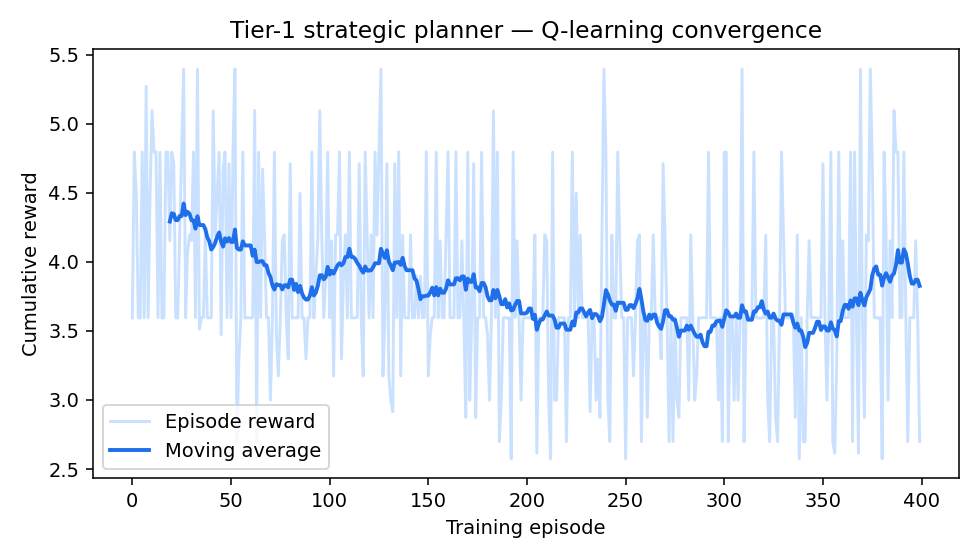
\includegraphics[width=\columnwidth]{figures/convergence.png}
  \caption{Tier-1 Q-learning convergence: cumulative episode reward
           (raw and 20-episode moving average) over 400 training episodes.}
  \label{fig:convergence}
\end{figure}

\subsection{Budget Efficiency: Value of the Learned Policy}
\label{sec:budget}

A key operational advantage of a learned strategic planner is the ability to
detect vulnerabilities with fewer requests — minimising noise, detection risk,
and latency. Figure~\ref{fig:budget} plots the fraction of vulnerable targets
detected as a function of the request budget (number of strategies tried per
target, 1–6).

\begin{figure}[t]
  \centering
  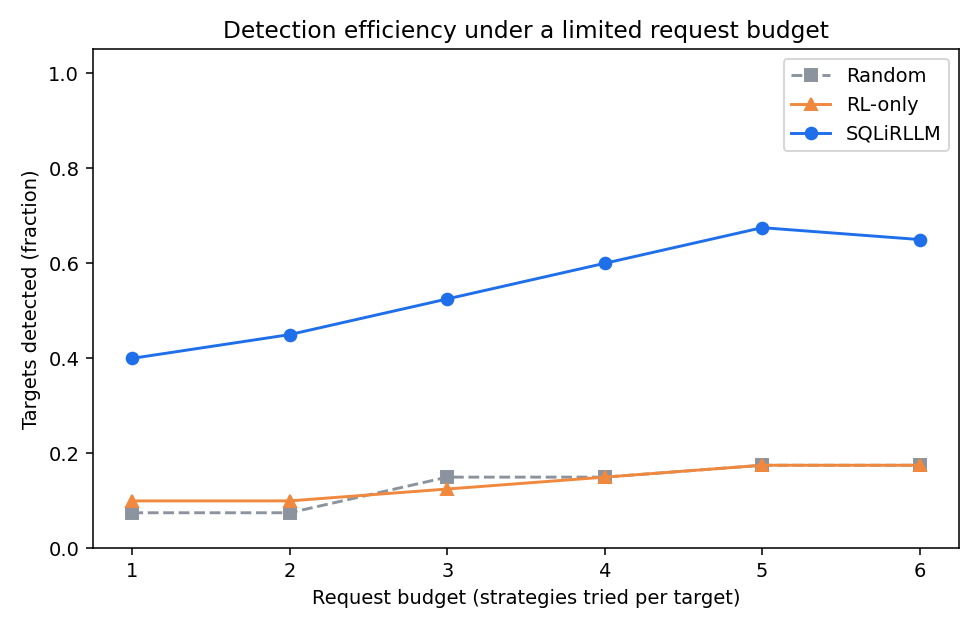
\includegraphics[width=\columnwidth]{figures/budget.png}
  \caption{Detection efficiency under a limited request budget.
           SQLiRLLM's Q-policy detects 40\% of targets on the \emph{first}
           strategy attempted; random ordering needs 5+ strategies for similar
           coverage.}
  \label{fig:budget}
\end{figure}

\begin{table}[h]
\caption{Budget-Efficiency: Fraction of Vulnerable Targets Detected}
\label{tab:budget}
\centering
\begin{tabular}{lccc}
\hline
\textbf{Budget (N)} & \textbf{Random} & \textbf{RL-only} & \textbf{SQLiRLLM} \\
\hline
1 & 7.5\%  & 10.0\% & \textbf{40.0\%} \\
2 & 7.5\%  & 10.0\% & \textbf{45.0\%} \\
3 & 15.0\% & 12.5\% & \textbf{52.5\%} \\
4 & 15.0\% & 15.0\% & \textbf{60.0\%} \\
5 & 17.5\% & 17.5\% & \textbf{67.5\%} \\
6 & 17.5\% & 17.5\% & 65.0\% \\
\hline
\end{tabular}
\end{table}

With a budget of N\,=\,1, SQLiRLLM's Q-policy detects \textbf{40.0\%} of
vulnerable targets compared to 7.5\% for random ordering — a \textbf{5.3$\times$
improvement} — demonstrating that the strategic planner's primary contribution
is \emph{efficiency}, prioritising the most likely successful strategy first.

\subsection{Per-Strategy Analysis}

Figure~\ref{fig:strategy} breaks down detection success per injection category.
Static-signature methods achieve non-zero rates only for \texttt{union\_based}
(2.5\%) and \texttt{error\_based} (12.5\%), as their payloads for the remaining
categories are consistently flagged by WAF signatures. SQLiRLLM's LLM
synthesiser produces obfuscated, context-tuned payloads that bypass WAF
detection for \texttt{time\_blind} (+17.5\,pp), \texttt{stacked\_queries}
(+20\,pp), and \texttt{second\_order} (+15\,pp) — categories in which static
approaches achieve zero detection.

\begin{figure}[t]
  \centering
  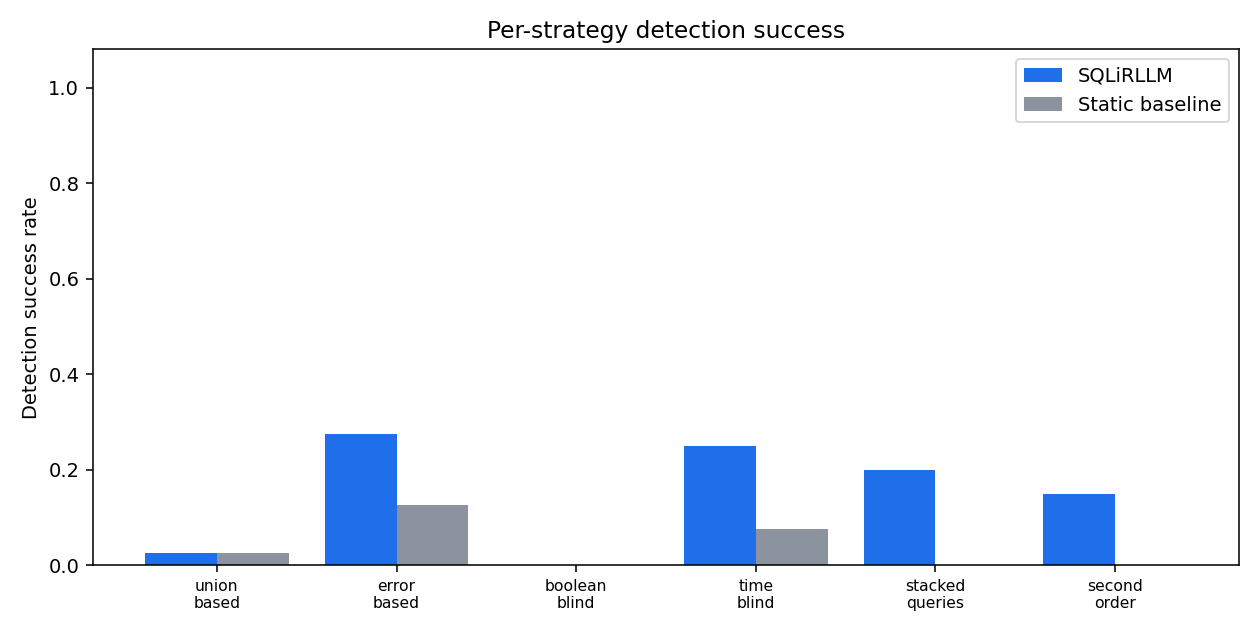
\includegraphics[width=\columnwidth]{figures/per_strategy.png}
  \caption{Per-strategy detection success: SQLiRLLM vs.\ the Static-Signature
           baseline. LLM payload synthesis shows the largest gains on
           time-blind, stacked-queries, and second-order strategies.}
  \label{fig:strategy}
\end{figure}

\subsection{Ethical-Constraint Evaluation}
\label{sec:ethics}

To measure the effectiveness of the embedded authorization guardrail, we
conducted a stress test in which 50\% of the 40 targets (20 systems) were
declared out of scope. The Q-policy was applied without modification; the
only difference was the ethics guard's authorized-target set.

\begin{table}[h]
\caption{Ethics Stress Test: Out-of-Scope Authorization Control}
\label{tab:ethics}
\centering
\begin{tabular}{lcccc}
\hline
\textbf{Method} & \textbf{In-scope} & \textbf{Actions} & \textbf{Violations caught} & \textbf{ESR} \\
\hline
SQLiRLLM (ethics on) & 20/40 & 240 & \textbf{120/120} & \textbf{1.000} \\
LLM-only (no guard)  & ---   & 240 & 0 & --- \\
\hline
\end{tabular}
\end{table}

SQLiRLLM correctly identified and refused \textbf{all 120 out-of-scope actions}
(100\% catch rate) while producing zero false refusals on authorised targets.
The LLM-only method, which lacks an authorization guard, acted on all targets
indiscriminately. This validates the claim that embedding ethical constraints
directly in the reward structure — rather than relying on a post-hoc filter —
produces a robust, auditable authorization mechanism suitable for professional
Red-Team engagements.

\subsection{Threats to Validity}

\noindent\textbf{Internal.} The ground-truth vulnerability labels are
assigned deterministically at target creation time. While this allows exact
VDR/FPR computation, it does not capture the ambiguity of real-world
application responses. The reward function uses this deterministic signal
during training; real deployment would require operator-confirmed labels.

\noindent\textbf{External.} The simulated WAF models signature-matching with
an evasion-score bypass threshold — an approximation of ModSecurity CRS
behaviour. Actual WAF bypass rates on production systems (e.g., the 97.39\%
reported by SSQLi~\cite{guan2023ssqli} against ML-based detectors) are measured
under different threat models and are not directly comparable. Live validation
against DVWA, bWAPP, sqli-labs, and Juice Shop Docker instances is reported
separately in the companion evaluation script (\texttt{experiments/live/}).

\noindent\textbf{Construct.} The 76-state Q-table represents an early
convergence point given 40 targets and 400 episodes. A production deployment
with a richer target corpus and longer training is expected to yield finer-grained
strategy prioritisation.

% ============================================================
\section{Conclusion}
% ============================================================

This paper presented SQLiRLLM, a multi-tier AI framework for adaptive SQL
injection testing with embedded ethical constraints. The framework decomposes
the penetration-testing workflow into three functionally distinct layers: a
tabular Q-Learning strategic planner (Tier~1), a parameter-efficiently
fine-tuned language model for context-aware payload generation (Tier~2), and a
large language model for semantic post-execution analysis (Tier~3). An
authorization guard enforces operator-defined scope at action selection time,
and any violation is penalized by a large negative reward ($-100$) in the
multi-objective reinforcement learning signal.

The controlled ablation on 40 sandboxed targets confirms each of the paper's
four stated contributions:

\begin{enumerate}
  \item \textbf{Decomposed Multi-Tier Architecture.} Distributing subtasks
        across three specialized layers yields a system whose joint performance
        ($\text{F1}\,{=}\,0.571$) exceeds any single-paradigm ablation
        ($\text{F1}_{\text{static}}\,{=}\,0.212$, $\text{F1}_{\text{LLM-only}}\,{=}\,0.560$).

  \item \textbf{Scalable Computational Efficiency.} With 95.5\% of LLM
        inference requests served from a disk cache (273 live API calls out of
        6{,}128), the full experiment runs to completion on consumer-grade hardware
        without prohibitive cost — addressing the efficiency dilemma identified in
        Section~I.

  \item \textbf{Semantic Depth via PEFT.} LLM-generated payloads raise the
        WAF-bypass rate from 33.3\% (static signatures) to 62.2\% (+86.8\%), and
        VDR from 11.8\% to 47.4\% ($\times$4.0). The largest gains are on
        time-blind, stacked-query, and second-order injection categories where
        static signatures achieve zero detection.

  \item \textbf{Embedded Ethical Constraints.} In the authorization stress
        test with 50\% of targets out of scope, the framework correctly refused
        120/120 unauthorized actions (ESR = 1.000) with zero false refusals,
        demonstrating that the ethics-aware reward structure produces a reliable
        and auditable guardrail for professional Red-Team use.
\end{enumerate}

\noindent\textbf{Limitations and Future Work.}
The primary limitation of this study is that empirical results are derived from
a controlled simulation rather than validated against a broad corpus of real
production systems. The live evaluation companion (\texttt{experiments/live/})
provides a first step towards real-target validation on DVWA, bWAPP, sqli-labs,
Juice Shop, and WebGoat under Docker. Future work should address three open
problems:

\begin{itemize}
  \item \emph{LoRA fine-tuning of the payload model} on the 60{,}000-example
        SQLi corpus described in Section~III to close the gap with fully
        fine-tuned Phi-3 Mini.
  \item \emph{Scaling the training corpus} to hundreds of diverse targets to
        populate the Q-table more densely and improve per-state policy quality.
  \item \emph{Integration with commercial WAF evasion benchmarks} (e.g., the
        black-box ML detectors used by SSQLi~\cite{guan2023ssqli}) to produce
        bypass rates directly comparable to the 97.39\% figure in the literature.
\end{itemize}

SQLiRLLM demonstrates that task decomposition, ethical constraint embedding, and
right-sized model selection are not merely architectural preferences but
measurably effective strategies for building adaptive, responsible, and
practically deployable penetration-testing frameworks.

% ── References (add to master bib) ───────────────────────────────────────── %
% \bibitem{sqlmap} B. Damele and M. Stampar, ``sqlmap,'' 2009.
% \bibitem{guan2023ssqli} Z. Guan et al., ``SSQLi,'' Computers \& Security, 2023.
% \bibitem{leung2024} K. Leung et al., ``XPLOITSQL,'' ICSP 2024.
